\subsection{Прямая}

\begin{wrapfigure}{r}{0.35\tw}
    \centering
    \vspace{-.8pc}
    \tikzsetnextfilename{math-line}
    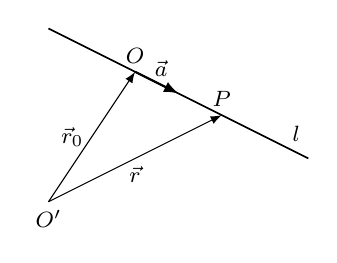
\begin{tikzpicture}[scale=1.1]
        \footnotesize
        \coordinate (O) at (0, 0);
        \coordinate (A) at (1, 1.5);
        \coordinate (B) at (2, 1);
        \coordinate (C) at (1.5, 1.25);
        \coordinate (L1) at (0, 2);
        \coordinate (L2) at (3, 0.5);


        \draw[-latex] (O) -- (A);
        \draw[-latex] (O) -- (B);
        \draw[thick, -latex] (A) -- (C);

        \draw[semithick] (L1) -- (L2);

        \point (O);
        \point (A);
        \point (B);

        \draw (O) node[anchor=north]{$O'$};
        \draw (A) node[anchor=south]{$O$};
        \draw (B) node[anchor=south]{$P$};

        \draw (1, 0.5) node[anchor=north]{$\vec{r}$};
        \draw (0.5, 0.75) node[anchor=east]{$\vec{r}_0$};
        \draw (1.3, 1.35) node[anchor=south]{$\vec{a}$};
        \draw (3, 0.6) node[anchor=south east]{$l$};
    \end{tikzpicture}
    \caption{}
    \label{pic:math-line}
\end{wrapfigure}
Рассмотрим необходимое условие, чтобы произвольная точка~$P$ с радиус-вектором~$\vec{r}$ лежала на прямой~$l$, проходящей через точку~$O$ с радиус вектором $\vec{r}_0$ (\lookPicRef{pic:math-line}). Пусть $ \vec{a} = \begin{pmatrix} a_1 & \cdots & a_n\end{pmatrix}^{\T}$~--- направляющий вектор прямой $l$, то есть $l$ параллельна прямой, содержащей вектор $\vec{a}$, тогда формально данное условие можно записать так:
\begin{equation}
    \vec{r} = \vec{r}_0 + \lambda \vec{a},\quad \lambda \in \R.
\end{equation}
Конкретизируем для случая векторов из $\R^2$:
\begin{gather*}
    \vec{r} - \vec{r}_0 = \lambda \vec{a} \quad \Rightarrow \quad
    \begin{cases}
        x - x_0 = \lambda x_a,\\
        y - y_0 = \lambda y_a.
    \end{cases}
\end{gather*}
Решив данную систему уравнений, получим, что
\begin{equation*}
    \lambda = \frac{x - x_0}{x_a} = \frac{y - y_0}{y_a}.
\end{equation*}
преобразуем второе равенство:
\begin{gather*}
    \frac{1}{x_a} \cdot x + \left( - \frac{1}{y_a} \right) \cdot y + \left( \frac{y_0}{y_a} - \frac{x_0}{x_a} \right) = 0,\\
    y_a x + (-x_a)y + (x_a y_0 - y_a x_0) = 0,
\end{gather*}
Сделав замену $y_a \equiv A$, $-x_a \equiv B$, $x_a y_0 - y_a x_0 \equiv C$, получим \imp{каноническое уравнение прямой на плоскости в декартовых координатах}:
\begin{equation}
    Ax + By + C = 0.
\end{equation}
Заметим, что
\begin{equation*}
    \scalar{a}{n} \equiv \scalar{a}{
    \begin{pmatrix}
        A\\
        B
    \end{pmatrix}} = x_a y_a - y_a x_a = 0,
\end{equation*}
значит, $\vec{n} \perp \vec{a}$, то есть вектор $\vec{n}$ есть вектор нормали к прямой с направляющим вектором $\vec{a}$, так как коэффициенты $A$ и $B$ не зависят от фиксированной точки $O$.
